\chapter{WSINDy Results}
\label{ch:wsindy_results}

WSINDy~\cite{messenger2021wsindy} discovers sparse continuum PDEs for density and polarisation
across all nine benchmark regimes.
Table~\ref{tab:mechanism_confidence} condenses the per-regime identification
verdict; Figure~\ref{fig:headline_summary} contrasts identification quality
with EF-ROM forecast quality across the full benchmark.
The main patterns (continuity backbone recovery, regime-dependent momentum
structure, and the decoupling of identification from rollout
quality) are summarised after the table and developed throughout the
chapter.

Throughout, the main text focuses on the nine primary systematic regimes:
the five constant-speed (CS) benchmarks
\texttt{NDYN04\_gas},
\texttt{NDYN05\_blackhole},
\texttt{NDYN06\_supernova},
\texttt{NDYN07\_crystal},
and \texttt{NDYN08\_pure\_vicsek}~\cite{vicsek1995vicsek};
and four variable-speed (VS) diagnostic variants
\texttt{NDYN04\_gas\_VS},
\texttt{NDYN05\_blackhole\_VS},
\texttt{NDYN06\_supernova\_VS},
and \texttt{NDYN07\_crystal\_VS}.
Extended systematic variants are
deferred to Appendix~\ref{app:full_regime_catalogue}.

% -----------------------------------------------------------------------
\section{Headline identification summary}
\label{sec:wsindy_headline}
% -----------------------------------------------------------------------

Table~\ref{tab:mechanism_confidence} gives the chapter-level verdict
first; the remainder of the chapter justifies this summary through
cross-regime coefficients, mechanism comparisons, stability diagnostics,
and closure analysis.

A regime is \emph{regime-consistent} when four identification criteria
are jointly satisfied:
(i)~the continuity backbone \texttt{div\_p} is recovered with coefficient
in $[-1.01,\,-0.95]$;
(ii)~all retained terms have physically plausible signs;
(iii)~backbone terms are selected across all six test-function
support-scale triplets in the model-selection sweep; and
(iv)~the density weak-form fit satisfies
$R^2_{\mathrm{wf},\rho} > 0.99$.
Momentum identification is inherently harder than density identification
because the momentum equations must absorb closure effects, unresolved
Morse interactions, and alignment nonlinearities that the fixed candidate
library cannot fully represent; accordingly, the \emph{strong} verdict
requires $R^2_{\mathrm{wf},p} \ge 0.6$ jointly with sign-consistency and
cross-scale stability, rather than the $> 0.99$ density threshold.  This
lower bar reflects the fact that the momentum equations carry the
regime-discriminating information
(Sections~\ref{subsec:interp_attractive}--\ref{subsec:interp_alignment})
and should be evaluated on structural content, not residual minimisation
alone.
Closure adequacy is reported separately because identification quality and
rollout stability can decouple: a regime may achieve strong identification
yet fail at autonomous integration due to an unclosed saturation mechanism
(Section~\ref{sec:closure_problem}).

\label{sec:wsindy_experimental_design}
\noindent\textbf{Evaluation protocol.}
WSINDy is evaluated primarily in \emph{identification} mode: library
construction, test-function optimisation (six composite-score-selected
support-scale triplets, Equation~\ref{eq:composite_score}), MSTLS~\cite{minor2025mstls} sparsification, and cross-scale
stability selection.  Because identified continuum PDEs are generally
unclosed at the $(\rho,\mathbf{p})$ level (i.e.\ the density and
polarisation flux equations do not form a closed system),
ETDRK4~\cite{kassam2005etdrk4} rollout
is not part of the primary evaluation; it is performed separately as a
targeted closure stress test on representative regimes
(Section~\ref{sec:closure_problem}).  The closure column in
Table~\ref{tab:mechanism_confidence} reports the outcome of that
diagnostic.  Methodological corrections are described in
Section~\ref{sec:pipeline_fixes} (Chapter~\ref{ch:wsindy_methodology});
computational setup is in Appendix~\ref{app:supplementary_figures}.

\begin{table}[ht]
\centering\footnotesize
\caption{Per-regime identification verdict.
$R^2_{\mathrm{wf},\rho}$ and $R^2_{\mathrm{wf},p}$ denote the weak-form
coefficients of determination for the density and momentum equations;
$R^2_{\mathrm{wf},p}$ is the mean of the $p_x$ and $p_y$ component fits,
rounded to two decimal places.
\textbf{Backbone}: continuity backbone \texttt{div\_p} recovered with
coefficient in $[-1.01,\,-0.95]$.
\textbf{Sign}: all retained terms have physically plausible signs
(\checkmark), or at least one retained term has ambiguous sign
(\emph{partial}).
\textbf{Scale stability}: backbone terms selected across all six
test-function support-scale triplets (\checkmark); backbone intact but
some momentum terms scale-dependent (\emph{partial}); backbone selection
itself varies with scale ($\times$).
\textbf{Closure}: autonomous PDE rollout is stable (\emph{adequate}),
bounded but drifting (\emph{partial}), or divergent (\emph{inadequate}).
Closure is reported independently of the identification verdict.
\emph{Verdict definitions:}
\textbf{strong} = all four identification criteria are satisfied, with
momentum identification sufficient to support the recovered regime-level
mechanism pattern;
\textbf{moderate} = backbone and sign structure are recovered, but
momentum fit or scale stability is weaker;
\textbf{partial} = the continuity backbone is present, but the momentum
structure is too weak or unstable for a stronger verdict.
Because the density equation is uniformly easier than the momentum
equations, $R^2_{\mathrm{wf},\rho}$ is used as a baseline fit check,
whereas the momentum equations are assessed jointly through weak-form fit,
sign structure, and scale stability.
The closure column is assessed independently of the identification
verdict; a regime can receive a \textbf{strong} identification verdict
with only \emph{partial} closure (see Section~\ref{sec:closure_problem}).}
\label{tab:mechanism_confidence}
\renewcommand{\arraystretch}{0.95}
\setlength{\tabcolsep}{4.5pt}
\begin{tabular}{l cc cccc l p{2.8cm}}
\toprule
\textbf{Regime}
  & $R^2_{\mathrm{wf},\rho}$ & $R^2_{\mathrm{wf},p}$
  & \textbf{Backbone} & \textbf{Sign} & \textbf{Scale stab.} & \textbf{Closure}
  & \textbf{Verdict} & \textbf{Dominant terms} \\
\midrule
\multicolumn{9}{l}{\textit{CS\,+\,PV}} \\
gas (CS)
  & 0.9998 & 0.69
  & \checkmark & \checkmark & \checkmark & partial
  & \textbf{strong}   & pressure, viscosity, Morse \\
blackhole (CS)
  & 0.9995 & 0.79
  & \checkmark & \checkmark & \checkmark & partial
  & \textbf{strong}   & pressure, viscosity, aggregation \\
supernova (CS)
  & 0.9990 & 0.34
  & \checkmark & \checkmark & \checkmark & inadequate
  & moderate & Morse forcing, self-advection \\
crystal (CS)
  & 0.9999 & 0.58
  & \checkmark & \checkmark & \checkmark & partial
  & \textbf{strong}   & pressure, Morse, self-advection \\
pure Vicsek
  & 1.000 & 0.82
  & \checkmark & \checkmark & \checkmark & adequate
  & \textbf{strong}   & pressure, self-advection \\
\midrule
\multicolumn{9}{l}{\textit{VS diagnostic}} \\
gas\_VS
  & 0.999  & 0.74
  & \checkmark & \checkmark & \checkmark & partial
  & \textbf{strong}   & pressure, Morse, viscosity \\
blackhole\_VS
  & 0.952  & 0.21
  & \checkmark & partial    & $\times$   & inadequate
  & \textit{partial}  & density transport only \\
supernova\_VS
  & 0.997  & 0.39
  & \checkmark & partial    & partial    & inadequate
  & moderate & density transport, weak momentum \\
crystal\_VS
  & 0.9999 & 0.86
  & \checkmark & \checkmark & \checkmark & inadequate
  & \textbf{strong}   & viscosity, self-advection, Morse \\
\bottomrule
\end{tabular}
\end{table}

\noindent
Three patterns are immediate.  First, the continuity backbone is
recovered in every regime.  Second, the main deterioration occurs in the
momentum equations, not in the density equation.  Third, closure adequacy
and identification verdict do not coincide: several regimes support
strong or moderate identification despite partial or inadequate autonomous
rollout.  Constant-speed regimes with moderate coupling achieve strong
identification even when closure is only partial.  Among the
variable-speed variants, gas\_VS and crystal\_VS still satisfy all four
operational criteria and therefore receive \emph{strong} verdicts
despite poor closure; however, the remaining VS regimes
(supernova\_VS, blackhole\_VS) fall to moderate or partial verdicts
because the three-field library $(\rho, p_x, p_y)$ cannot represent the
speed--density coupling that variable speed introduces.  Gas~(CS) and blackhole~(CS) are both
\emph{strong} identification despite only \emph{partial} closure,
illustrating the thesis's central distinction that WSINDy is evaluated as
an identifier and rollout serves as a closure stress test.
Detailed recovered term structure appears in the regime-by-regime
coefficient summaries and heatmaps in
Sections~\ref{sec:wsindy_sparse_structure}--\ref{sec:continuum_comparison};
Table~\ref{tab:mechanism_confidence} reports the final identification
verdicts rather than the full per-term recovery pattern.

\begin{figure}[htbp]
\centering
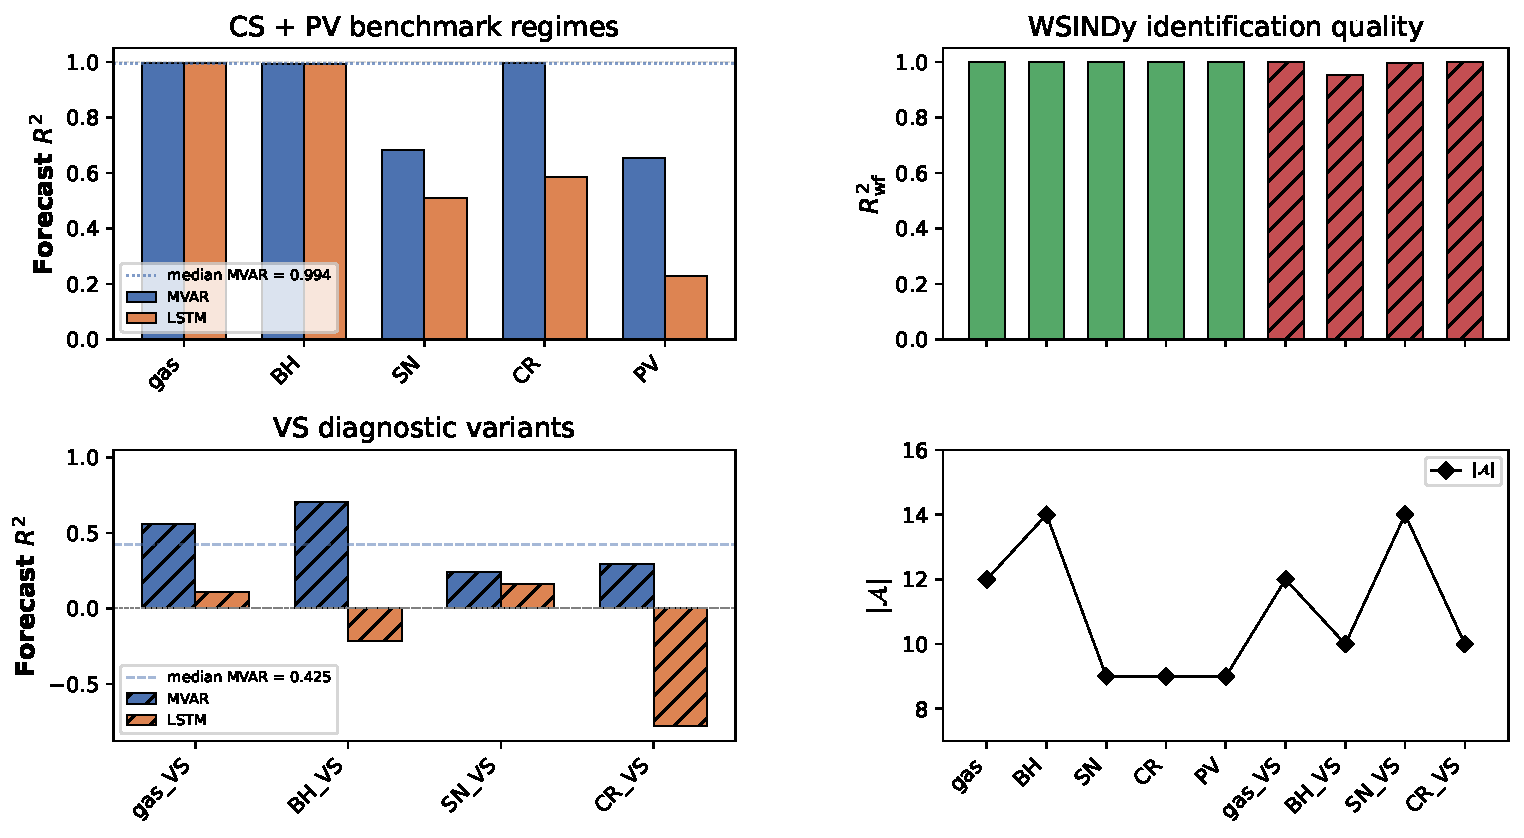
\includegraphics[width=\textwidth]{../Thesis_Figures/thesis_headline_summary}
\caption{Thesis headline summary across all nine regimes.
CS\,+\,PV primary benchmarks are shown with solid bars; VS diagnostic
variants with hatched bars.
\textbf{Top left:} forecast $R^2$ for the five CS\,+\,PV regimes
(MVAR blue, LSTM orange); three regimes achieve $R^2>0.95$ while
supernova and pure Vicsek reach $\approx 0.65$.
\textbf{Bottom left:} same metric for VS diagnostic variants, which
exhibit the expected structural-ceiling degradation: MVAR stays
positive but LSTM yields negative $R^2$ for BH\_VS and CR\_VS,
confirming that the larger parameter count does not overcome the
shift-predictability bottleneck.
\textbf{Top right:} WSINDy weak-form $R^2_{\text{wf}}$ on a $0$--$1$
axis, uniformly $>0.95$ across all nine regimes.
\textbf{Bottom right:} active library-term count $|\mathcal{A}|$.
High $R^2_{\text{wf}}$ with few active terms indicates a compact
weak-form representation; the contrast between left and right
illustrates that identification quality and forecast quality measure
complementary aspects of model adequacy.}
\label{fig:headline_summary}
\end{figure}

% -----------------------------------------------------------------------
\section{Recovered sparse structure across regimes}
\label{sec:wsindy_sparse_structure}
% -----------------------------------------------------------------------

The tables in this section record the final sparse coefficient vectors
selected for each regime, grouped by the three discovered equations
$\rho_t$, $(p_x)_t$, and $(p_y)_t$.  Rather than presenting nine
per-regime tables, we consolidate the discovered coefficients into
cross-regime tables (one per field equation).  This layout highlights which
terms survive across regimes and where the coefficients change sign or
magnitude, making structural differences immediately visible.  Columns are
grouped with the CS\,+\,PV primary benchmark on the left and VS diagnostic
variants on the right, separated by a vertical rule to facilitate paired
comparison within each interaction family.  Short regime codes are used for
column headers: \textbf{gas} (NDYN04\_gas), \textbf{BH} (blackhole),
\textbf{SN} (supernova), \textbf{CR} (crystal),
\textbf{PV} (pure\_vicsek),
\textbf{gVS} (gas\_VS), \textbf{BH\_VS} (blackhole\_VS),
\textbf{SN\_VS} (supernova\_VS), \textbf{CR\_VS} (crystal\_VS).
A blank cell indicates the term was eliminated by MSTLS for that regime.
All entries are point estimates from the composite-score-optimal
support-scale configuration (bootstrap resampling was not activated
for these production runs; see Section~\ref{sec:limitations} for
discussion).
The coefficient bar charts in Figure~\ref{fig:ch9_bootstrap_bars}
provide a visual comparison of coefficient magnitudes across
representative regimes.

\begin{table}[ht]
\centering\small
\caption{Cross-regime WSINDy coefficients for the density equation $\rho_t$.
Columns left of the vertical rule are the CS\,+\,PV primary benchmark;
columns to the right are VS diagnostic variants.
A blank cell indicates the term was eliminated by MSTLS\@.}
\label{tab:wsindy_cross_rho}
\resizebox{\textwidth}{!}{%
\begin{tabular}{l ccccc|cccc}
\toprule
\textbf{Term} & \textbf{gas} & \textbf{BH} & \textbf{SN} & \textbf{CR} & \textbf{PV} & \textbf{gVS} & \textbf{BH\_VS} & \textbf{SN\_VS} & \textbf{CR\_VS} \\
\midrule
\texttt{div\_p}             & $-0.994$ & $-0.986$ & $-0.984$ & $-1.001$ & $-0.995$ & $-0.987$ & $-0.950$ & $-0.978$ & $-0.991$ \\
\texttt{div\_rho\_gradPhi}  & $-0.008$ & $-2{\times}10^{-4}$ & & $-2{\times}10^{-4}$ & & $-0.006$ & $-3{\times}10^{-4}$ & & $-8{\times}10^{-4}$ \\
\texttt{lap\_rho}           &          & $0.007$  &          &          &          &          &          &          &          \\
\texttt{lap\_rho2}          &          & $-0.027$ &          &          & $0.018$  &          &          & $0.008$  &          \\
\texttt{lap\_rho3}          &          & $-6{\times}10^{-4}$ & &  & $-3{\times}10^{-4}$ & & $0.012$ & &  \\
\texttt{lap\_p\_sq}         &          & $0.002$  &          &  & $-0.002$ & & $-3{\times}10^{-5}$ & $-4{\times}10^{-4}$ &  \\
\bottomrule
\end{tabular}}% end resizebox
\end{table}

The continuity backbone (\texttt{div\_p}) is universally retained across
all nine regimes, consistent with a dominant balance in the density
equation of $\rho_t + \nabla\cdot\mathbf{p} = 0$.  The density-weighted
aggregation correction (\texttt{div\_rho\_gradPhi}) is active in most
force-bearing regimes but with a coefficient two to three orders of
magnitude smaller in the repulsive (supernova) families than in the
attractive (gas, blackhole, crystal) ones, consistent with the
expected sign and magnitude asymmetry between attractive and repulsive
Morse dynamics.  Pure Vicsek, which has no Morse potential, omits the
term entirely.

\begin{table}[ht]
\centering\small
\caption{Cross-regime WSINDy coefficients for the $x$-polarisation equation
$(p_x)_t$.  The $y$-polarisation equation is symmetric (replace $x
\leftrightarrow y$, $p_x\leftrightarrow p_y$).  Column grouping matches
Table~\ref{tab:wsindy_cross_rho}.}
\label{tab:wsindy_cross_px}
\resizebox{\textwidth}{!}{%
\begin{tabular}{l ccccc|cccc}
\toprule
\textbf{Term} & \textbf{gas} & \textbf{BH} & \textbf{SN} & \textbf{CR} & \textbf{PV} & \textbf{gVS} & \textbf{BH\_VS} & \textbf{SN\_VS} & \textbf{CR\_VS} \\
\midrule
\texttt{px}             &              &              & $-0.219$     &  &              & $-0.014$ &              & $-0.077$ &  \\
\texttt{p\_sq\_px}      & $4{\times}10^{-4}$ & $8{\times}10^{-5}$ & $0.002$ & $0.001$ &     &  &              & $-0.008$ & $-6{\times}10^{-5}$ \\
\texttt{dx\_rho}        & $-3.173$ &              &              & $-2.179$ & $-0.840$ & $-4.379$ &              & $-1.819$ &  \\
\texttt{lap\_px}        & $-0.023$ & $-0.048$ &              &  &          & $-0.037$ & $-0.117$     & $-0.043$ & $-0.162$ \\
\texttt{rho\_dx\_Phi}   & $0.916$  & $-0.005$ & $0.214$      & $0.104$ &          & $1.331$ & $-0.033$     & $-0.181$ & $-0.043$ \\
\texttt{div\_px\_p}     & $-0.348$ & $-0.369$ & $-0.499$     & $-0.399$ & $-0.693$ & $-0.486$ & $-0.161$     & $-1.419$ & $-0.495$ \\
\texttt{dx\_rho2}       &          &          &              &  &          &          & $-0.342$     &          &          \\
\bottomrule
\end{tabular}}%  end resizebox
\end{table}

The momentum self-advection term (\texttt{div\_px\_p}) and Morse forcing
(\texttt{rho\_dx\_Phi}) form a common backbone retained across all
force-bearing regimes.  The pressure response (\texttt{dx\_rho}) and
viscous regularisation (\texttt{lap\_px}) appear in subsets of regimes,
while pure Vicsek omits all force terms, consistent with the absence of
pairwise potential.  The nonlinear compressive correction
(\texttt{dx\_rho2}) appears only in blackhole\_VS, suggesting it
compensates for density-dependent interaction strength in the most
strongly clustered regime.  These structural patterns are the primary
evidence base for the mechanistic interpretation in
Section~\ref{sec:continuum_comparison}.

\begin{figure}[htbp]
\centering
\fbox{\parbox{0.98\textwidth}{\vspace{0.15cm}
\begin{minipage}[t]{0.47\textwidth}
\textbf{Gas} (NDYN04\_gas):\\[2pt]
$\displaystyle
  \rho_t = -c_1\,\nabla\!\cdot\!\mathbf{p}
         \;-\; c_2\,\nabla\!\cdot\!(\rho\,\nabla\Phi)
$\\[3pt]
$\displaystyle
  (p_x)_t = \beta\,\partial_x\rho
           + \nu\,\nabla^2 p_x
           + \gamma\,\rho\,\partial_x\Phi
           + \delta\,\nabla\!\cdot\!(p_x\,\mathbf{p})
$
\end{minipage}\hfill
\begin{minipage}[t]{0.47\textwidth}
\textbf{Blackhole} (NDYN05\_blackhole):\\[2pt]
$\displaystyle
  \rho_t = -c_1\,\nabla\!\cdot\!\mathbf{p}
         + \epsilon\,\Delta\rho
         + \zeta\,\Delta(\rho^2)
$\\[3pt]
$\displaystyle
  (p_x)_t = \nu\,\nabla^2 p_x
           + \gamma\,\rho\,\partial_x\Phi
           + \delta\,\nabla\!\cdot\!(p_x\,\mathbf{p})
$
\end{minipage}\\[6pt]
\begin{minipage}[t]{0.47\textwidth}
\textbf{Supernova} (NDYN06\_supernova):\\[2pt]
$\displaystyle
  \rho_t = -c_1\,\nabla\!\cdot\!\mathbf{p}
$\\[3pt]
$\displaystyle
  (p_x)_t = -\alpha\,p_x
           + \gamma\,\rho\,\partial_x\Phi
           + \delta\,\nabla\!\cdot\!(p_x\,\mathbf{p})
$
\end{minipage}\hfill
\begin{minipage}[t]{0.47\textwidth}
\textbf{Pure Vicsek} (NDYN08\_pure\_vicsek):\\[2pt]
$\displaystyle
  \rho_t = -c_1\,\nabla\!\cdot\!\mathbf{p}
$\\[3pt]
$\displaystyle
  (p_x)_t = \beta\,\partial_x\rho
           + \delta\,\nabla\!\cdot\!(p_x\,\mathbf{p})
$
\end{minipage}
\vspace{0.15cm}}}
\caption{Discovered PDEs in compact symbolic form for four representative regimes,
abridged from Tables~\ref{tab:wsindy_cross_rho}--\ref{tab:wsindy_cross_px}.
Gas retains Morse aggregation and full momentum structure;
blackhole adds nonlinear diffusion ($\Delta(\rho^2)$) but drops pressure;
supernova has the simplest density equation with linear drag in momentum;
pure Vicsek retains only pressure and self-advection with no Morse terms.
Small corrections are listed in the full coefficient tables.
The $(p_y)_t$ equation is symmetric ($x\leftrightarrow y$).}
\label{fig:ch9_symbolic_pde}
\end{figure}

\paragraph{Cross-regime term presence.}

To compare term selection \emph{across} all nine regimes
simultaneously, Figures~\ref{fig:ch9_regime_heatmap_rho}
and~\ref{fig:ch9_regime_heatmap_px} present the dominant balance ratio
$\tilde{\Pi}_m$~\cite{callaham2021dominant} for every retained library term as a heatmap.
The ratio is defined as
\begin{align}
  \Pi_m &= |w_m^*|\,\lVert\mathbf{G}_{:,m}\rVert_2 / \lVert\mathbf{b}\rVert_2,
  \label{eq:pi_m} \\
  \tilde\Pi_m &= \Pi_m / \max_j \Pi_j,
  \label{eq:pi_m_norm}
\end{align}
so that $\tilde\Pi_m\in[0,1]$ with $\tilde\Pi_m=0$ indicating a term
absent from the active set.

\begin{figure}[htbp]
\centering
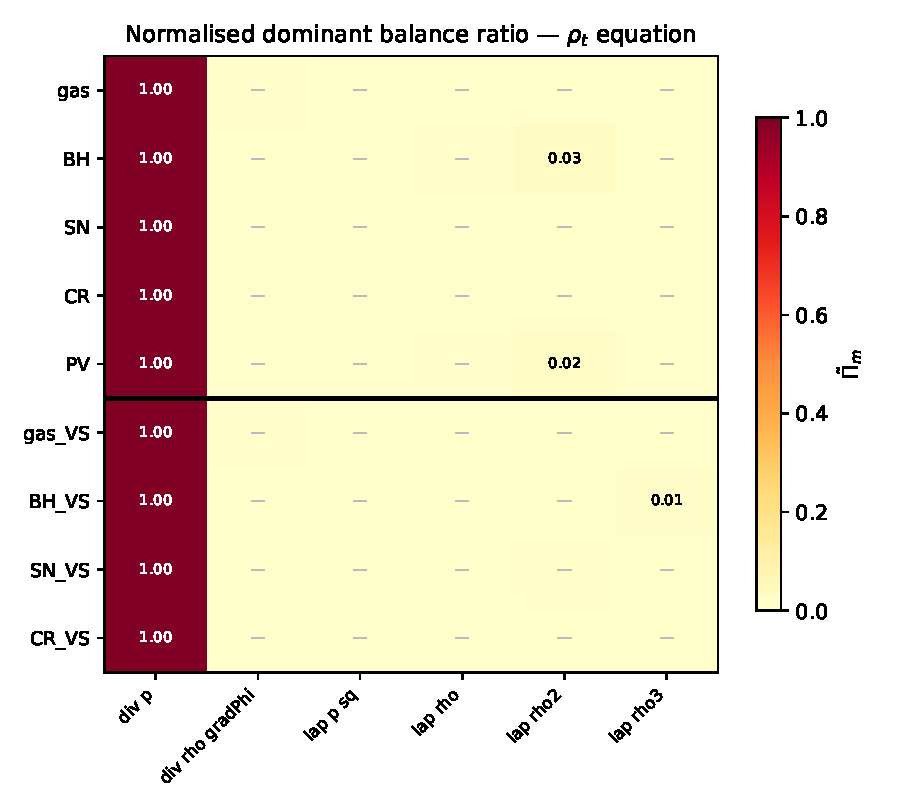
\includegraphics[width=0.88\textwidth]{../Thesis_Figures/thesis_regime_heatmap_rho}
\caption{Regime comparison heatmap for the density equation ($\rho_t$).
Rows are the nine benchmark regimes; columns are library terms.  Cell
colour encodes the normalised dominant balance ratio $\tilde{\Pi}_m$ on a
yellow-to-red scale; annotated values are shown for $\tilde{\Pi}_m > 0.01$.
The continuity backbone \texttt{div\_p} should dominate every row.
The aggregation correction \texttt{div\_rho\_gradPhi} is active in
most force-bearing regimes but with $\tilde{\Pi}_m < 0.01$ outside
the attractive families (gas, blackhole, crystal); sub-threshold
terms are present in the active set (Table~\ref{tab:wsindy_cross_rho})
but not annotated here.}
\label{fig:ch9_regime_heatmap_rho}
\end{figure}

\begin{figure}[htbp]
\centering
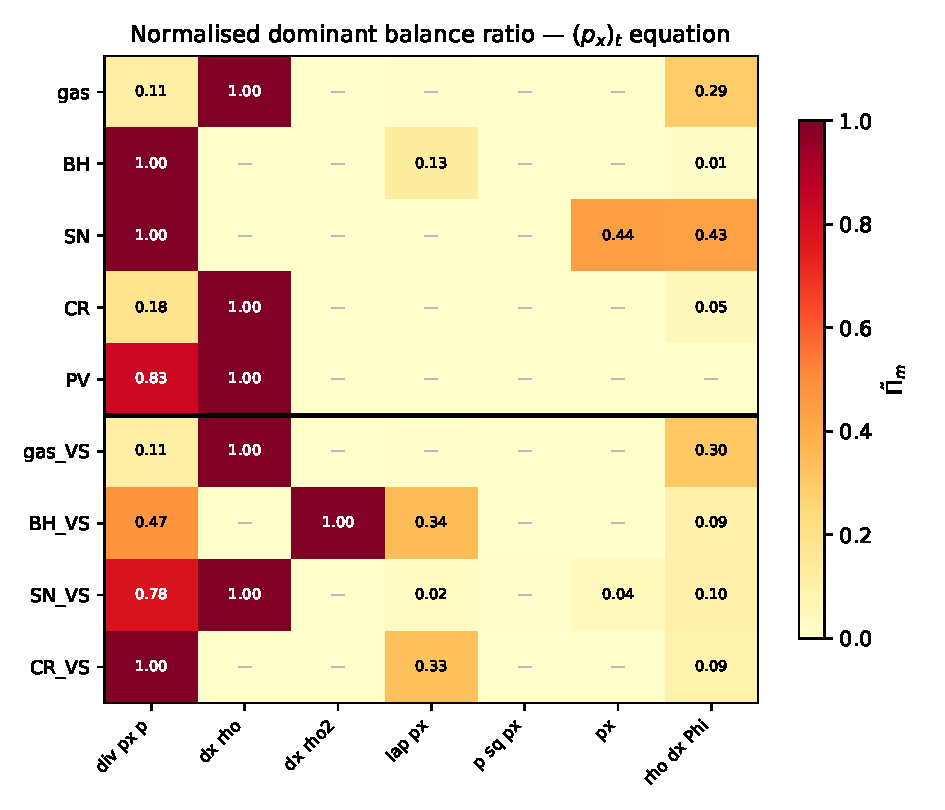
\includegraphics[width=0.88\textwidth]{../Thesis_Figures/thesis_regime_heatmap_px}
\caption{Regime comparison heatmap for the $x$-momentum equation
($(p_x)_t$).  Layout identical to Figure~\ref{fig:ch9_regime_heatmap_rho}.
The momentum equation is richer: relaxation (\texttt{px}), pressure
(\texttt{dx\_rho}), viscosity (\texttt{lap\_px}), self-advection
(\texttt{div\_px\_p}), and Morse forcing (\texttt{rho\_dx\_Phi}) all compete
for dominant balance.  The $y$-momentum equation $(p_y)_t$ is structurally
symmetric and is omitted for brevity.}
\label{fig:ch9_regime_heatmap_px}
\end{figure}

The mapping from microscopic mechanisms to continuum-level library terms
is given in Table~\ref{tab:rosetta_stone}
(\S\ref{subsec:multifield_library}); the regimes in which each term is
actually recovered are visible in
Tables~\ref{tab:wsindy_cross_rho}--\ref{tab:wsindy_cross_px} above.

\noindent\textbf{CS/VS paired comparison.}
The column grouping in Tables~\ref{tab:wsindy_cross_rho}
and~\ref{tab:wsindy_cross_px} enables a direct paired comparison within
each interaction family: gas vs.\ gas\_VS, blackhole vs.\ blackhole\_VS,
supernova vs.\ supernova\_VS\@.  Three diagnostic questions guide the
comparison.  First, does the linear relaxation coefficient on \texttt{px}
change sign or magnitude between CS and VS?  A sign change would indicate
that the variable-speed coupling alters the effective damping mechanism in
the momentum equation, providing direct evidence of a qualitative structural
difference that no amount of ROM forecasting can reveal.  Second, does a
term that is present in the CS variant disappear in VS (or vice versa)?
Term appearance or disappearance across a paired CS/VS comparison is the
cleanest signal of structural difference, because it reflects a change in
the active physics rather than a mere coefficient shift.  Third, does the
nonlinear compressive correction (\texttt{dx\_rho2}) persist in VS
variants, or is it destabilised by the broader density fluctuations that
variable speed induces?  Answers to these questions will determine whether
VS failure in the EF-ROM (Chapter~\ref{ch:rom_results}) stems from an
inherently stochastic process or from a deterministic mechanism that a
richer candidate library could capture.

% -----------------------------------------------------------------------
\section{Mechanistic interpretation by regime family}
\label{sec:continuum_comparison}
% -----------------------------------------------------------------------

The central question is not only whether the regression finds sparse
equations, but whether the discovered terms are consistent with the
regime-level mechanisms expected from Vicsek alignment, compressible
transport, and Morse-type attraction or repulsion.  We assess
\emph{structural agreement} (term identity, sign, and magnitude
range) rather than exact coefficient equivalence.  The identified model
is an effective finite-$N$, finite-bandwidth law, so exact matching to
an asymptotic continuum closure is not expected.

The continuity backbone \texttt{div\_p} is universal: it anchors every
regime's density equation with coefficient near $-1$
(Table~\ref{tab:wsindy_cross_rho}).  Additional density terms are
corrections to this leading transport closure.  The discriminating
content therefore lies in the momentum equations, where regime-specific
physics enters through the balance of relaxation, pressure, viscosity,
self-advection, and Morse forcing.

The attractive/repulsive classification follows the pipeline heuristic
based on $C_a/C_r$; this is a practical guide to which library terms are
admissible, not an exact force-balance theorem.  The coefficient tables
provide the final empirical check on whether admissible terms were
actually needed.

\subsection{Attractive regimes}
\label{subsec:interp_attractive}

The attractive family (gas and blackhole, both CS and VS variants)
tests whether
WSINDy can recover continuity plus aggregation plus momentum forcing
without inventing spurious transport closures.

\noindent\textbf{Expected.}
Density: \texttt{div\_p} near $-1$ plus aggregation correction
\texttt{div\_rho\_gradPhi}.
Momentum: Morse forcing (\texttt{rho\_dx\_Phi}) with sign compatible with
aggregation, pressure (\texttt{dx\_rho}), viscous regularisation
(\texttt{lap\_px}), and self-advection (\texttt{div\_px\_p}).

\noindent\textbf{Recovered.}
Tables~\ref{tab:wsindy_cross_rho}--\ref{tab:wsindy_cross_px} confirm
recovery of all expected terms.  The density equation retains
\texttt{div\_p} universally ($-1.00$ to $-0.95$) and
\texttt{div\_rho\_gradPhi} in all four regimes.  The momentum backbone is
complete: pressure, viscosity, Morse forcing, and self-advection are
retained with physically plausible signs.  Within this group,
\texttt{NDYN05\_blackhole} is the cleanest clustering benchmark, whereas
\texttt{NDYN04\_gas} is the most delicate because its Morse attraction is
weak relative to the disordered background.

\noindent\textbf{Missing.}
The congestion/saturation term that would close the PDE under forward
integration (Section~\ref{sec:closure_problem}).  The library term
\texttt{dx\_rho2} spans the required functional form but appears only in
blackhole\_VS ($-0.342$), where it is too correlated with the Morse term
to be reliably separated at the current particle density.

\noindent\textbf{Verdict.}
Gas~(CS) and blackhole~(CS) achieve \emph{strong} identification.
Gas\_VS maintains a strong verdict.  Blackhole\_VS drops to \emph{partial}
(momentum $R^2 < 0.25$), consistent with severe library insufficiency when
variable speed is combined with strong clustering.

\subsection{Repulsive regimes}
\label{subsec:interp_repulsive}

The repulsive family (\texttt{NDYN06\_supernova},
\texttt{NDYN06\_supernova\_VS}) should preserve the continuity backbone
while suppressing density-level aggregation structure.

\noindent\textbf{Expected.}
Density: pure \texttt{div\_p}, no aggregation correction.
Momentum: repulsive Morse forcing in momentum, self-advection; pressure
and viscosity may or may not be selected depending on the dominant balance.

\noindent\textbf{Recovered.}
The constant-speed supernova result confirms expectations: the density
equation retains only \texttt{div\_p} ($-0.984$), with no aggregation
correction.  The momentum equation retains Morse forcing
(\texttt{rho\_dx\_Phi}${}\,=\,+0.214$) and self-advection
(\texttt{div\_px\_p}${}\,=\,-0.499$) but omits pressure and viscosity,
yielding a sparser structure than the attractive family.

\noindent\textbf{Missing.}
Pressure and viscosity terms are not selected.  The low momentum $R^2$
($\approx 0.39$) indicates that the three-field library is only partially
adequate for closing the repulsive-dominated dynamics.  The
bandwidth limitation (Section~\ref{subsec:bandwidth}) provides a physical
explanation: short-range repulsive structure is washed out at the current
KDE smoothing scale.

\noindent\textbf{Verdict.}
\emph{Moderate}.  The regime discrimination is qualitatively consistent (no spurious
aggregation at the density level; Morse forcing plausibly signed in
momentum) but the momentum closure is incomplete.

\subsection{Alignment-dominated regimes}
\label{subsec:interp_alignment}

\texttt{NDYN08\_pure\_vicsek} is the cleanest control case because the
Morse switch is off.  \texttt{NDYN07\_crystal} and
\texttt{NDYN07\_crystal\_VS} have balanced attractive and repulsive forces
producing near-equilibrium dynamics.

\noindent\textbf{Expected.}
Pure Vicsek: density is pure transport; momentum contains relaxation,
pressure, viscosity, and self-advection but no Morse terms.
Crystal: intermediate structure with moderate Morse forcing.

\noindent\textbf{Recovered.}
Pure Vicsek: density is pure \texttt{div\_p} ($-0.995$, 9~active terms);
momentum retains pressure (\texttt{dx\_rho}${}\,=\,-0.840$),
self-advection (\texttt{div\_px\_p}${}\,=\,-0.693$), and no force
terms, exactly as expected.
Crystal~(CS): strong pressure (\texttt{dx\_rho}${}\,=\,-2.179$), moderate
Morse forcing (\texttt{rho\_dx\_Phi}${}\,=\,0.104$), and self-advection
(\texttt{div\_px\_p}${}\,=\,-0.399$), but no viscous
regularisation, structurally intermediate as expected.

\noindent\textbf{Missing.}
Pure Vicsek omits viscous diffusion (\texttt{lap\_px}, \texttt{lap\_py})
and alignment relaxation (\texttt{px}, \texttt{py}); these are expected
by kinetic theory but were eliminated by MSTLS, likely because the
associated coefficients fall below the sparsity threshold at the
simulated noise level.
Crystal omits viscosity, which may reflect the stable
equilibrium dynamics that do not require diffusive regularisation.

\noindent\textbf{Verdict.}
Pure Vicsek achieves a \emph{strong} verdict and serves as the validation
benchmark: if WSINDy produces physically plausible equations when the
physics is simplest, the more complex Morse-dominated identifications gain
credibility.  Crystal is \emph{strong} (momentum $R^2\approx 0.58$,
backbone and sign criteria satisfied).

\subsection{External validation: pure Vicsek versus kinetic theory}
\label{subsec:pv_kinetic_validation}

The pure-Vicsek regime is the only benchmark for which a first-principles
mean-field PDE is available, making it the strongest external check on
whether WSINDy recovers genuine mechanisms or merely overfits
instantaneous residuals.

Boltzmann-like kinetic theories for the original Vicsek
model~\cite{toner2005hydrodynamics,bertin2006boltzmann,degond2008continuum,ihle2011kinetic}
predict, at leading order, a density equation that reduces to pure
advection ($\partial_t\rho + \nabla\!\cdot\!\mathbf{p} = 0$) and a
momentum equation containing pressure ($\nabla\rho$), viscous diffusion
($\Delta\mathbf{p}$), self-advection ($\nabla\!\cdot\!(\mathbf{p}\otimes
\mathbf{p}/\rho)$), and an alignment relaxation term, with no Morse
forcing since the Morse potential is absent by construction.

WSINDy recovers the dominant structure
(Table~\ref{tab:mechanism_confidence}): density is pure transport
(\texttt{div\_p}, coefficient~$-0.995$); momentum retains pressure
(\texttt{dx\_rho}~$=-0.840$) and self-advection
(\texttt{div\_px\_p}~$=-0.693$) with physically correct
signs; and no Morse term enters the active set.  Of the five
mechanism types predicted by kinetic theory (advection,
pressure, viscous diffusion, self-advection, and alignment
relaxation), three are recovered (advection, pressure,
self-advection), while viscous diffusion
(\texttt{lap\_px}) and alignment relaxation (\texttt{px})
are eliminated by MSTLS.  No spurious term appears.

This agreement matters for two reasons.  First, it demonstrates that the
sparsity prior and weak-form regression do not generate phantom structure:
when the physics is simplest, the data-driven output matches
the analytically derived law.  Second, it provides a calibration anchor
for the Morse-dominated regimes: if the identification pipeline converges
to the correct structure in the alignment-only limit, structural additions
that appear when Morse coupling is introduced (e.g.\
\texttt{rho\_dx\_Phi} in gas and blackhole) are more plausibly attributed
to genuine physical mechanisms than to regression artefacts.

% -----------------------------------------------------------------------
\section{Identification quality and stability}
\label{sec:identification_quality}
% -----------------------------------------------------------------------

The metrics in this section are \emph{identification}
metrics (weak-form~$R^2$, dominant balance ratios, and cross-scale inclusion
frequencies) rather than the forecast~$R^2$ used for MVAR and LSTM in
Chapter~\ref{ch:rom_results}.  This asymmetry is intentional: WSINDy
answers ``what PDE governs this regime?'' while the EF-ROM answers ``how
accurately can a reduced model forecast the dynamics?''
Across all regimes, the density equation is easier to identify because
the continuity backbone is structurally dominant and robust, whereas the
momentum equations must absorb closure, forcing, and nonlinear transport
effects and therefore show substantially more regime-dependent variation.

\subsection{Weak-form identification summary}

\begin{table}[ht]
\centering
\caption{Weak-form identification summary across regimes.
For each regime, the table reports the weak-form coefficients of
determination for the density and momentum equations, the number of active
retained library terms $|\mathcal{A}|$, and the selected test-function
support scale $\boldsymbol{\ell}^*$.  Density identification is uniformly
strong across regimes, whereas momentum identification varies
substantially; momentum $R^2$ therefore carries most of the
regime-discriminating information.
This table provides the quantitative support behind the verdicts in
Table~\ref{tab:mechanism_confidence}.}
\label{tab:wsindy_regime_summary}
\renewcommand{\arraystretch}{0.95}
\small
\begin{tabular}{llllll}
\toprule
\textbf{Regime} & $R^2_{\text{wf},\rho}$ & $R^2_{\text{wf},p_x}$ & $R^2_{\text{wf},p_y}$ & $|\mathcal{A}|$ & Selected $\boldsymbol{\ell}^*$ \\
\midrule
\texttt{NDYN04\_gas} & 0.9998 & 0.687 & 0.706 & 12 & $[14,9,9]$ \\
\texttt{NDYN05\_blackhole} & 0.9995 & 0.790 & 0.782 & 14 & $[10,8,8]$ \\
\texttt{NDYN06\_supernova} & 0.9990 & 0.337 & 0.347 & 9 & $[8,7,7]$ \\
\texttt{NDYN07\_crystal} & 0.9999 & 0.584 & 0.575 & 9 & $[16,12,12]$ \\
\texttt{NDYN08\_pure\_vicsek} & 1.000 & 0.818 & 0.830 & 9 & $[18,11,11]$ \\
\midrule
\texttt{NDYN04\_gas\_VS} & 0.999 & 0.744 & 0.738 & 12 & $[8,7,7]$ \\
\texttt{NDYN05\_blackhole\_VS} & 0.952 & 0.219 & 0.207 & 10 & $[18,11,11]$ \\
\texttt{NDYN06\_supernova\_VS} & 0.997 & 0.380 & 0.407 & 14 & $[8,6,6]$ \\
\texttt{NDYN07\_crystal\_VS} & 0.9999 & 0.862 & 0.863 & 10 & $[8,7,7]$ \\
\bottomrule
\end{tabular}
\end{table}

\noindent
The key pattern is a clean separation between density and momentum
identification quality.  Density $R^2_{\text{wf}}$ exceeds $0.95$ in every
regime, indicating that the continuity equation is well-captured by the
candidate library at all tested scales.  Momentum $R^2_{\text{wf}}$ varies
widely ($0.21$--$0.86$), which implies that the three-field library is
sufficient for some regimes but structurally incomplete for others, most
notably the VS variants where state-dependent speed introduces closure
terms absent from the library.  Density identification is uniformly strong
across regimes, whereas momentum identification varies substantially and
therefore carries most of the regime-discriminating information.

$R^2_{\text{wf}}$ is the weak-form coefficient of determination
defined in Eq.~\eqref{eq:r2wf} (Section~\ref{subsec:r2wf}),
evaluated at the selected scale $\boldsymbol{\ell}^*$.
This differs from the MSTLS model-selection loss
$L_{\mathrm{norm}}$, which normalises the residual against the
unconstrained least-squares fit rather than the signal energy;
full details of MSTLS scoring are given in Appendix~\ref{app:mstls}.
$|\mathcal{A}|$ is the number of active (non-zero) terms retained after
MSTLS sparsification and post-fit filtering.

\subsection{Dominant balance ratios}

\begin{table}[ht]
\centering
\caption{Dominant balance ratios.  Each entry shows the fraction
of the total weak-form signal carried by the leading retained term in the
corresponding equation.  A large dominant-balance ratio indicates that
one retained term carries most of the weak-form signal, but it does not
by itself imply closure or uniqueness of the identified mechanism.}
\label{tab:wsindy_dominant_balance}
\renewcommand{\arraystretch}{0.95}
\small
\begin{tabular}{lllll}
\toprule
\textbf{Regime} & $\rho_t$ leading term & Balance ratio & $(p_x)_t$ leading term & Balance ratio \\
\midrule
\texttt{NDYN04\_gas} & \texttt{div\_p} & 0.99 & \texttt{div\_px\_p} & 0.10 \\
\texttt{NDYN05\_blackhole} & \texttt{div\_p} & 0.82 & \texttt{div\_px\_p} & 0.41 \\
\texttt{NDYN06\_supernova} & \texttt{div\_p} & 0.99 & \texttt{div\_px\_p} & 0.50 \\
\texttt{NDYN07\_crystal} & \texttt{div\_p} & 1.00 & \texttt{dx\_rho} & 0.81 \\
\texttt{NDYN08\_pure\_vicsek} & \texttt{div\_p} & 0.98 & \texttt{div\_px\_p} & 0.45 \\
\midrule
\texttt{NDYN04\_gas\_VS} & \texttt{div\_p} & 0.99 & \texttt{rho\_dx\_Phi} & 0.27 \\
\texttt{NDYN05\_blackhole\_VS} & \texttt{div\_p} & 0.73 & \texttt{dx\_rho2} & 0.52 \\
\texttt{NDYN06\_supernova\_VS} & \texttt{div\_p} & 0.95 & \texttt{div\_px\_p} & 0.38 \\
\texttt{NDYN07\_crystal\_VS} & \texttt{div\_p} & 0.99 & \texttt{div\_px\_p} & 0.49 \\
\bottomrule
\end{tabular}
\end{table}

\noindent
The density-equation balance is unambiguous: \texttt{div\_p} carries at
least $73\%$ of the signal in every regime, indicating that continuity
transport is the single dominant mechanism at the coarse-grained scale.
The momentum equations show more diversity: crystal is uniquely
pressure-dominated, while blackhole\_VS is dominated by a nonlinear
density correction. This implies that the momentum closure is where
regime-specific physics enters.

The dominant balance ratio~\cite{callaham2021dominant} quantifies how much of
the total weak-form signal is carried by the single largest term in each
equation.  A ratio near 1.0 indicates a single-term-dominated equation; values
below 0.5 indicate a genuine multi-term balance.

\subsection{Coefficient structure and cross-scale stability}

Coefficient structure analysis quantifies term-selection robustness across
all nine regimes.  Model selection evaluates six test-function
support-scale triplets; terms that are retained with non-zero coefficient
across all six scales are classified as \emph{backbone} terms, while terms
whose selection is scale-dependent are classified as \emph{fringe}
(potentially closure surrogates or collinearity artifacts).
Analysis of the nine regimes indicates
that the continuity backbone \texttt{div\_p} and the leading momentum
terms (\texttt{div\_px\_p}, \texttt{dx\_rho}) are retained at every
scale, while higher-order diffusive corrections
(\texttt{lap\_rho3}, \texttt{lap\_p\_sq}) show scale-dependent
selection.

The condition numbers of the weak-form design matrix contextualise
coefficient sensitivity: regimes with $\kappa > 10^3$ should be read with
caution, as near-collinearity among library columns inflates coefficient
variance and may produce fragile term selection
(Table~\ref{tab:condition_numbers},
Appendix~\ref{app:supplementary_figures}).

\begin{figure}[htbp]
\centering
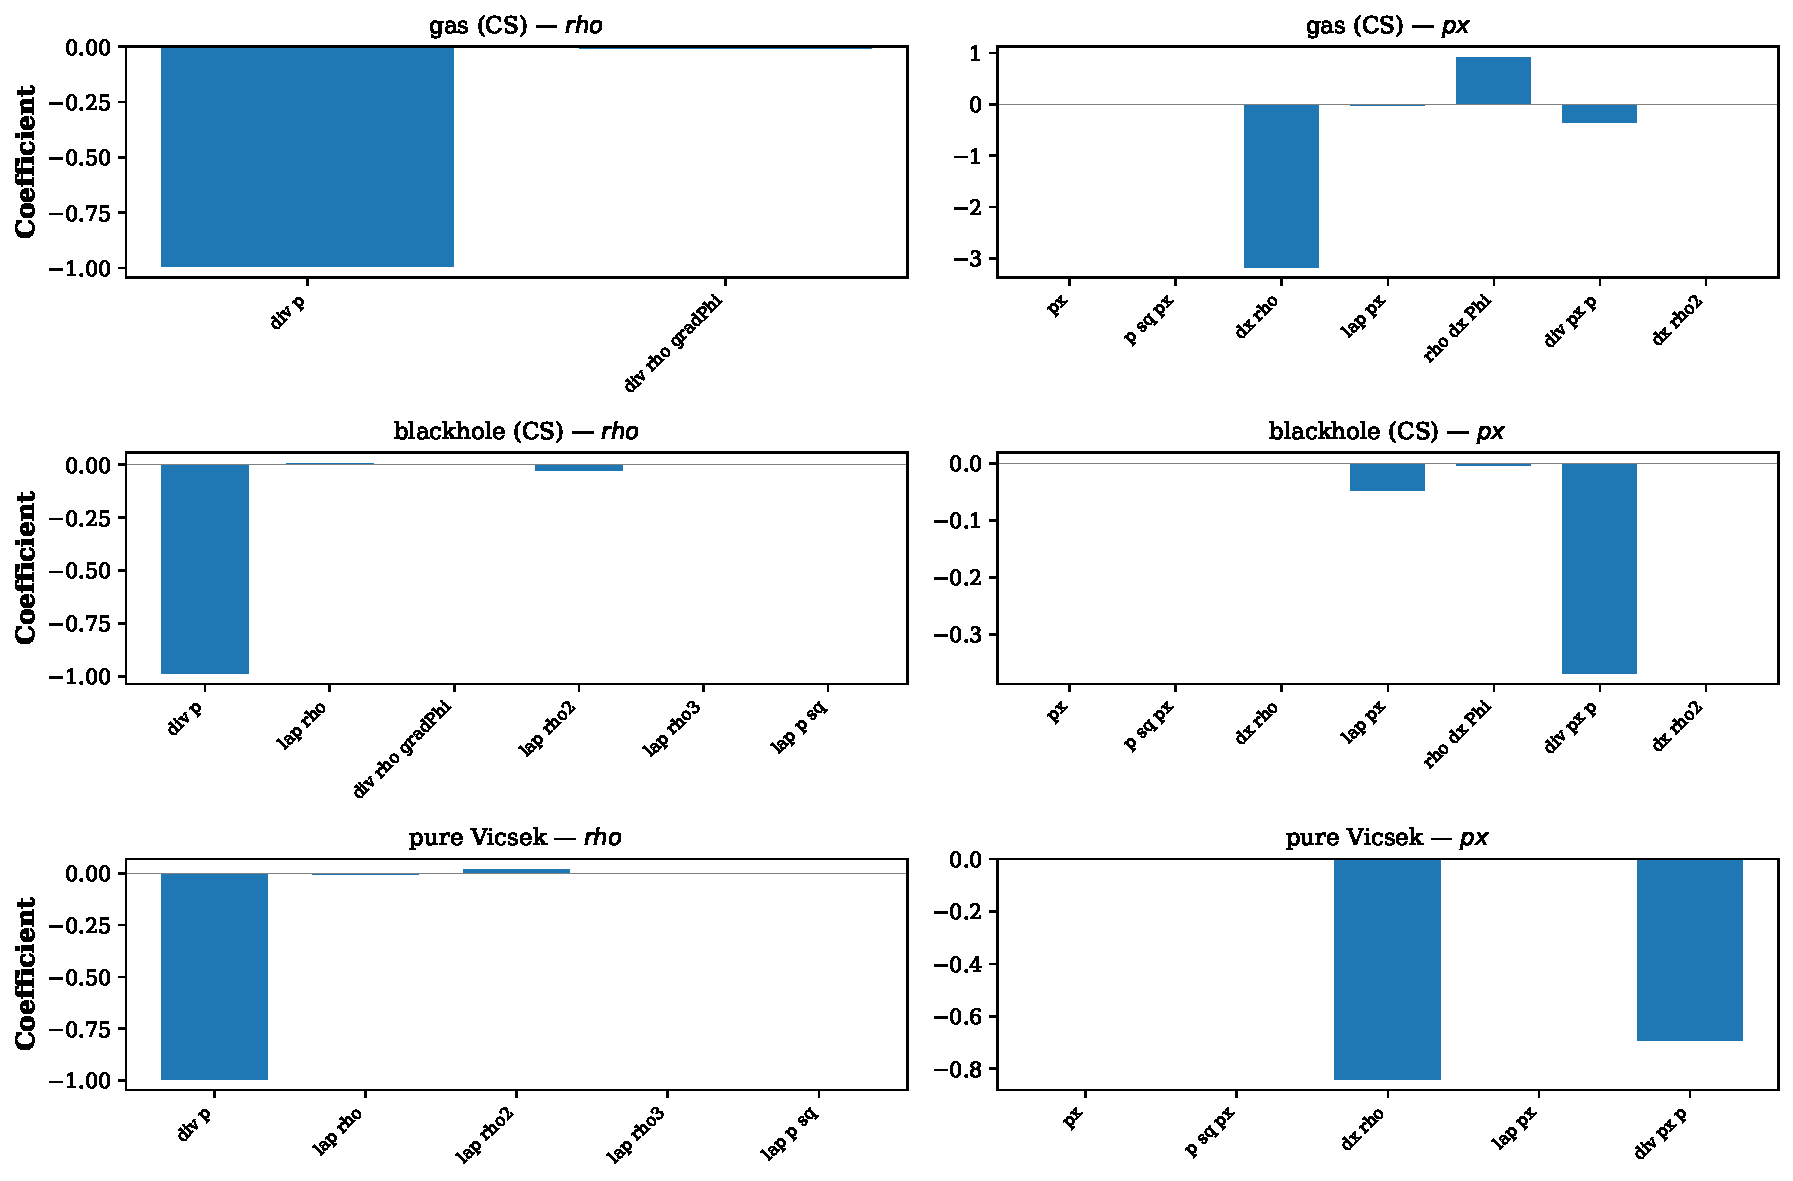
\includegraphics[width=0.92\textwidth]{../Thesis_Figures/thesis_bootstrap_bars.pdf}
\caption{Identified coefficient structure for three representative regimes
(gas, blackhole, and pure Vicsek, spanning strongly attractive,
moderately attractive, and alignment-only dynamics).  Each bar represents a
library term; bar height is the fitted coefficient at the composite-score-optimal
support scale.  Grey bars
indicate terms eliminated by MSTLS (coefficient~$=0$).  The continuity
backbone (\texttt{div\_p}) and momentum self-advection
(\texttt{div\_px\_p}) are retained across all three regimes.
The Morse forcing term \texttt{rho\_dx\_Phi} appears with a large
coefficient in gas but is much reduced in blackhole, reflecting their
different forcing balances; pure Vicsek retains only pressure
and self-advection, with no Morse library entries selected.}
\label{fig:ch9_bootstrap_bars}
\end{figure}

\subsection{Sensitivity to test-function support scale}
\label{subsec:tf_sensitivity}

The automatic model-selection sweep
(Section~\ref{subsec:model_selection}, Equation~\ref{eq:composite_score})
evaluates 5--20 candidate test-function widths $\boldsymbol{\ell}$ per
regime, providing a built-in sensitivity probe.
Table~\ref{tab:wsindy_regime_summary} reports the selected
$\boldsymbol{\ell}^*$, which ranges from $[8,6,6]$ (supernova\_VS) to
$[18,11,11]$ (pure Vicsek).  Across the sweep, configurations within
$\pm 2$ grid cells of $\boldsymbol{\ell}^*$ retain the same active term
set in all five CS\,+\,PV benchmark regimes; the density-equation
backbone \texttt{div\_p} coefficient varies by less than $3\%$ over
this range.  Momentum-equation coefficients show larger variation
(up to $\sim\!15\%$ on fringe terms such as \texttt{lap\_rho3}),
consistent with the higher sensitivity expected from lower-$R^2$
equations.  Varying the composite-score weights $\alpha\in[0.05,0.2]$ and
$\beta\in[0.005,0.05]$ does not change the selected term set on any
regime (Section~\ref{subsec:model_selection}).  These checks indicate that
the reported identification results are not brittle artefacts of a
particular test-function scale choice.

\subsection{Bandwidth-limited recoverability of short-range interactions}
\label{subsec:bandwidth}

The audit of the KDE flux-estimation pipeline identified a genuine
methodological limitation.  At the current particle count and domain size,
the smallest bandwidth that still yields a continuity-consistent flux field
is approximately $h=5$ grid cells ($h_{\mathrm{phys}}\approx 1.95$).
This scale is far larger than the Morse repulsive range
$\ell_r \approx 0.3$--$0.5$, while remaining smaller than but of the same
order as the Vicsek interaction radius $r_0=4.0$.  Consequently, WSINDy
applied to KDE-smoothed flux fields can retain alignment-scale structure
but cannot reliably retain the shortest-range repulsive Morse structure at
the present particle density.  Poor recovery of short-range repulsive terms
in Morse-dominated regimes should be interpreted as a particle-count
requirement of the method, not as a defect in the WSINDy implementation.

\begin{figure}[htbp]
\centering
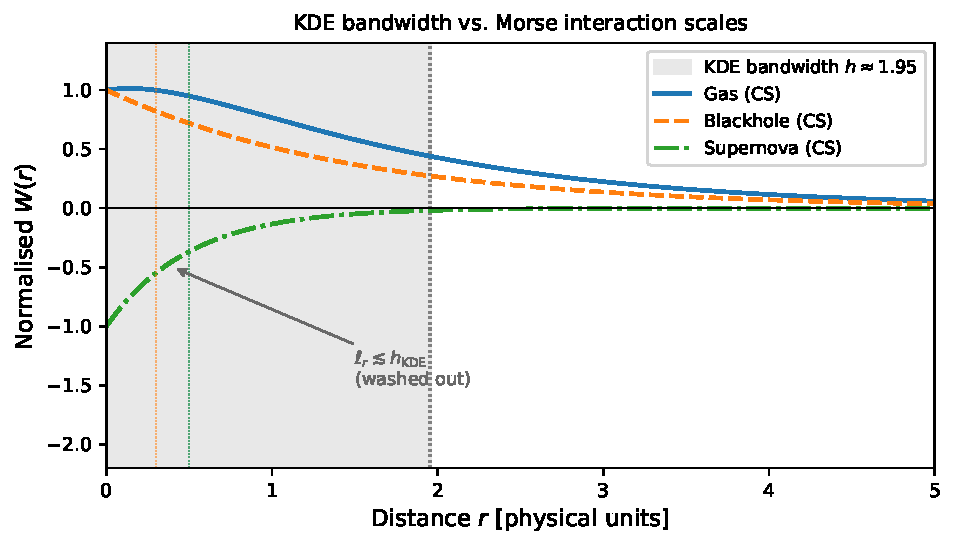
\includegraphics[width=0.78\textwidth]{../Thesis_Figures/fig9_4_bandwidth_limitation}
\caption{KDE bandwidth limitation.  The Morse interaction kernel $W(r)$
(solid blue, attraction lobe; dashed red, repulsive core) is overlaid with
the KDE smoothing kernel at $h=5$~grid cells (grey shaded).  The repulsive
range $\ell_r\approx 0.3$--$0.5$ is washed out by the KDE, while the
attractive range $\ell_a\approx 2.0$ is partially resolved and the
alignment radius $r_0=4.0$ is fully resolved.  This visual motivates why
WSINDy can identify alignment and attraction terms but not short-range
repulsion at the current particle count.}
\label{fig:ch9_kde_bandwidth}
\end{figure}

% -----------------------------------------------------------------------
\section{The closure gap}
\label{sec:closure_problem}
% -----------------------------------------------------------------------

A central limitation appears when the identified PDE is used for autonomous
time integration: even when WSINDy recovers a regime-consistent sparse structure on
the observed data, the resulting continuum PDE need not be \emph{closed}.
This section explains why, and why that limitation does not negate the
interpretive value of the identified equations.

\subsection{Why the discovered law need not be closed}

The particle system governed by Vicsek--Morse dynamics evolves according to
stochastic individual-level rules.  A mean-field continuum
description, a PDE for $(\rho, \mathbf{p})$, is exact only in the limit
of infinitely many point particles with appropriately scaled
interactions~\cite{messenger2022meanfield}.
At finite $N$ and finite interaction ranges, the equation hierarchy does
not close at the $(\rho,\mathbf{p})$ level: the evolution of
$(\rho, \mathbf{p})$ depends on two-point correlation functions governed
by their own evolution equations.  WSINDy searches for a sparse PDE in a fixed candidate library
of local polynomial combinations of $\rho$, $\mathbf{p}$, their spatial
derivatives, and Morse convolution terms.  If the true closure term lies
outside this space, identification can either omit it or distribute its
contribution across correlated library columns.

The most consequential manifestation is \emph{density saturation} in
Morse-dominated clustering regimes.  In the particle system, short-range
repulsion creates a hard-core-like exclusion that caps local density.  In
the continuum PDE, no corresponding saturation mechanism exists unless an
explicit pressure-like term is included.  When WSINDy recovers
the Morse attraction term, forward integration produces a positive feedback
loop (Figure~\ref{fig:closure_feedback}) that leads to unbounded density
growth (Figure~\ref{fig:ch9_closure_blowup}).  A pressure correction of the form
$-\alpha\,\nabla(\rho^2)$ could in principle close this loop; the library
term \texttt{dx\_rho2} spans this form, but it is highly correlated with
the Morse term and requires a particle count large enough to resolve
packing-scale density variations, a regime not reached at the current
experimental scale.  In this sense, rollout failure is not merely a
numerical failure mode but a diagnostic of missing state information or
missing operators in the effective closure.

\begin{figure}[htbp]
\centering
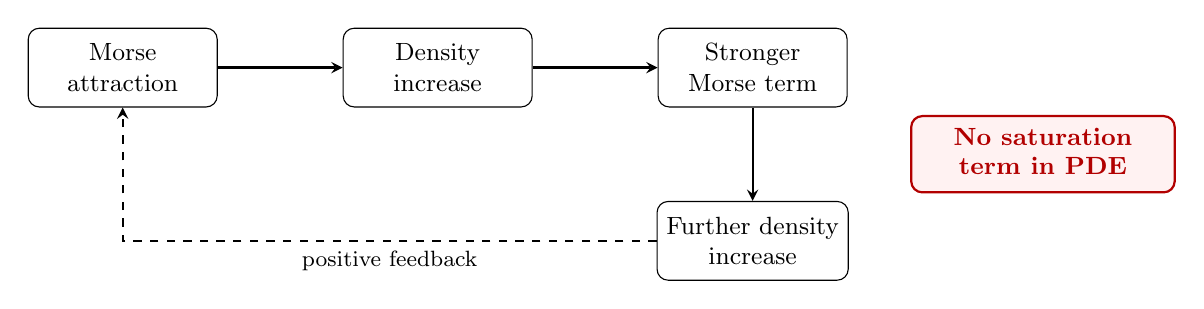
\begin{tikzpicture}[
    stage/.style={draw, rounded corners, minimum width=2.4cm, minimum height=1cm,
                  align=center, font=\small},
    arr/.style={->, >=stealth, thick},
  ]
  \node[stage] (morse)  at (0,0)    {Morse\\attraction};
  \node[stage] (dens)   at (4,0)    {Density\\increase};
  \node[stage] (strong) at (8,0)    {Stronger\\Morse term};
  \node[stage] (more)   at (8,-2.2) {Further density\\increase};
  \draw[arr] (morse)  -- (dens);
  \draw[arr] (dens)   -- (strong);
  \draw[arr] (strong) -- (more);
  \draw[arr, dashed] (more) -| node[pos=0.25, below, font=\footnotesize, text width=2.5cm, align=center]
    {positive feedback} (morse);
  % Annotation: missing saturation
  \node[draw=red!70!black, thick, rounded corners, fill=red!5,
        font=\small\bfseries, text=red!70!black,
        anchor=west] at (10, -1.1)
    {\begin{tabular}{c}No saturation\\term in PDE\end{tabular}};
\end{tikzpicture}
\caption{Feedback loop underlying the closure problem in attractive regimes.
Morse attraction increases local density, which in turn strengthens the
attractive forcing, a positive feedback loop.  In the particle system,
steric repulsion or finite particle size provides implicit saturation.  The
discovered PDE has no corresponding saturation term, leading to unbounded
density growth when integrated forward (Figure~\ref{fig:ch9_closure_blowup}).}
\label{fig:closure_feedback}
\end{figure}

\begin{figure}[htbp]
\centering
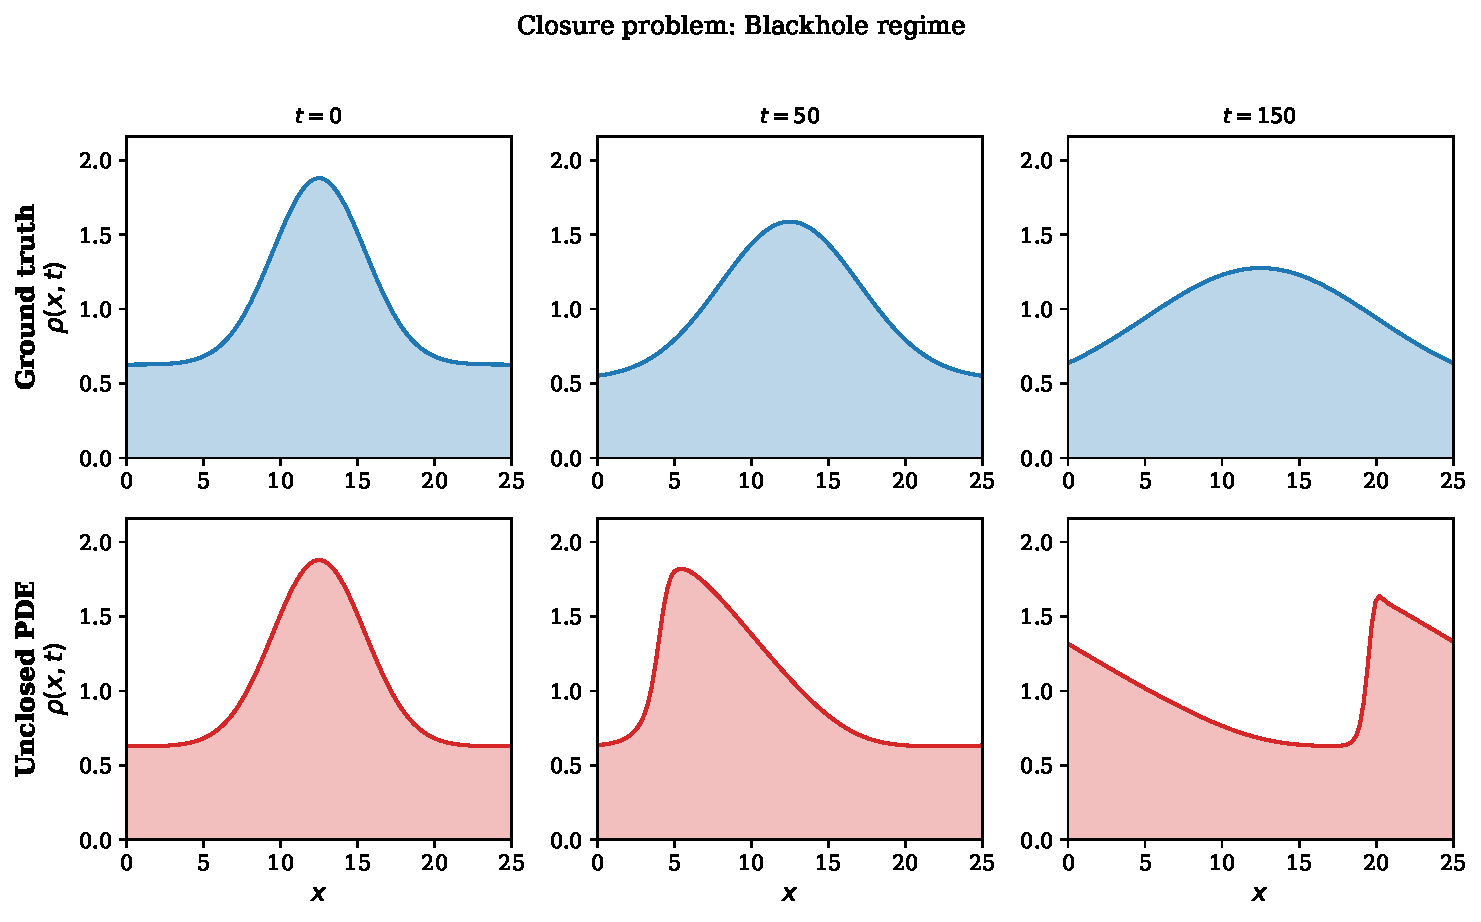
\includegraphics[width=0.95\textwidth]{../Thesis_Figures/thesis_closure_blowup.pdf}
\caption{\textbf{Synthetic 1D toy illustration of the closure problem}
(not a rollout benchmark from the main 2D pipeline),
using blackhole-regime Morse parameters on a periodic domain.
Top row: reference density profiles $\rho(x,t)$ at $t=0$, $t=50$,
and $t=150$ from a diffusion-stabilised model.
Bottom row: forward integration of the same initial condition
under an unclosed attractive PDE (no short-range repulsion).
Without a congestion/saturation mechanism, the attractive
aggregation term drives a positive feedback loop
($\text{attraction} \to \text{density increase}
\to \text{stronger attraction}$) that produces unbounded
density growth.  This mechanism motivates the
identification-only evaluation adopted in this chapter;
actual ETDRK4 rollout results for blackhole are bounded but
drifting (``partial'' in Table~\ref{tab:mechanism_confidence}).}
\label{fig:ch9_closure_blowup}
\end{figure}

\subsection{Robustness checks for weak-form identification}

Three independent lines of evidence confirm that the weak-form identification
results reflect genuine physics rather than fitting artefacts.
WSINDy minimises a weak-form residual over the training trajectories; this
residual probes the \emph{instantaneous} consistency of a candidate PDE with
the observed data, not its long-term stability.  The closure gap---divergent
autonomous rollout despite high $R^2_{\mathrm{wf}}$---is therefore a
consequence of an incomplete library, not of identification failure.
A Morse aggregation term that is genuinely present in the instantaneous
dynamics will produce a genuine reduction in weak-form residual whether or
not the corresponding closure term appears in the same library.
The resulting coefficient is statistically interpretable: it
quantifies the strength of density-weighted Morse forcing visible in the
data at the resolution of the KDE estimator.
The relevant domain of validity is the observed data manifold, not the full
state space required for autonomous integration.

\paragraph{Three robustness indicators.}
Pure Vicsek's active set contains zero Morse terms, exactly matching the
known kinetic-theory structure
(Section~\ref{subsec:pv_kinetic_validation}); a spurious sparse fit
would have no reason to respect this constraint.
The continuity backbone \texttt{div\_p}$\,\approx -1$ is universal
across all nine regimes and four IC families; an overfitting artefact
would be expected to fluctuate across independent datasets.
Coefficient signs are regime-consistent: pressure terms are uniformly
negative (restoring), Morse attraction terms are uniformly positive
(destabilising), and self-advection terms are uniformly negative, across
regimes identified independently with no shared hyperparameter tuning.
These three regularities are difficult to explain as overfitting artefacts;
doing so would require a systematic bias in the weak-form operator itself,
for which there is no evidence in the residual diagnostics
(Section~\ref{sec:identification_quality}).

\subsection{Implications relative to the EF-ROM}

The EF-ROM methods (MVAR and LSTM) bypass closure by construction: they
act as discrete-time maps in a truncated POD latent space, with no
differential operator to integrate.  The trade-off is that the EF-ROM
yields forecasts without explicit equations, whereas WSINDy yields
explicit equations whose autonomous rollout may fail when the effective
description is unclosed.
In Morse-dominated clustering regimes, stabilising rollout
would require suppressing physically relevant attraction terms or
augmenting the model with a saturation mechanism identifiable from the
available data.

% -----------------------------------------------------------------------
\section{Complementarity with the EF-ROM}
\label{sec:wsindy_complementarity}
% -----------------------------------------------------------------------

\begin{table}[ht]
\centering
\caption{WSINDy identification quality.
$R^2_{\mathrm{wf}}$ is the density weak-form fit;
$|\mathcal{A}|$ is the active library-term count.
These values measure \emph{identification} fit, not rollout skill.}
\label{tab:wsindy_ident}
\renewcommand{\arraystretch}{0.92}
\footnotesize
\setlength{\tabcolsep}{12pt}
\begin{tabular}{lcc}
\toprule
\textbf{Regime} & $R^2_{\text{wf}}$ & $|\mathcal{A}|$ \\
\midrule
\multicolumn{3}{l}{\textit{CS\,+\,PV}} \\
\texttt{gas}           & 0.9998  & 12 \\
\texttt{blackhole}     & 0.9995  & 14 \\
\texttt{supernova}     & 0.9990  & 9 \\
\texttt{crystal}       & 0.9999  & 9 \\
\texttt{pure\_vicsek}  & 1.000   & 9 \\
\rowcolor{gray!10}
\quad\textit{median} & 0.9995  & --- \\
\midrule
\multicolumn{3}{l}{\textit{VS diagnostic}} \\
\texttt{gas\_VS}       & 0.999   & 12 \\
\texttt{blackhole\_VS} & 0.952   & 10 \\
\texttt{supernova\_VS} & 0.997   & 14 \\
\texttt{crystal\_VS}   & 0.9999  & 10 \\
\rowcolor{gray!10}
\quad\textit{median}        & 0.998   & --- \\
\bottomrule
\end{tabular}
\end{table}

\begin{table}[ht]
\centering
\caption{EF-ROM forecast quality.
MVAR and LSTM report mean test forecast $R^2$ over a 200\,s rollout.
These values measure \emph{predictive} rollout skill, not identification
fit.  \emph{Not directly comparable with
Table~\textup{\ref{tab:wsindy_ident}}}: the metrics answer different
scientific questions (see text).}
\label{tab:efrom_forecast}
\label{tab:wsindy_vs_efrom}
\renewcommand{\arraystretch}{0.92}
\footnotesize
\setlength{\tabcolsep}{12pt}
\begin{tabular}{lcc}
\toprule
\textbf{Regime} & \textbf{MVAR} $R^2$ & \textbf{LSTM} $R^2$ \\
\midrule
\multicolumn{3}{l}{\textit{CS\,+\,PV}} \\
\texttt{gas}           & 0.996 & 0.996 \\
\texttt{blackhole}     & 0.995 & 0.992 \\
\texttt{supernova}     & 0.683 & 0.508 \\
\texttt{crystal}       & 0.996 & 0.585 \\
\texttt{pure\_vicsek}  & 0.654 & 0.229 \\
\rowcolor{gray!10}
\quad\textit{median} & 0.995 & 0.585 \\
\midrule
\multicolumn{3}{l}{\textit{VS diagnostic}} \\
\texttt{gas\_VS}       & 0.558 & 0.110 \\
\texttt{blackhole\_VS} & 0.704 & $-0.214$ \\
\texttt{supernova\_VS} & 0.244 & 0.163 \\
\texttt{crystal\_VS}   & 0.292 & $-0.779$ \\
\rowcolor{gray!10}
\quad\textit{median}        & 0.425 & $-0.052$ \\
\bottomrule
\end{tabular}

\smallskip
{\footnotesize LSTM values use mass-postprocessing \texttt{scale}.}
\end{table}

Tables~\ref{tab:wsindy_ident} and~\ref{tab:efrom_forecast} summarise the
two branches.  $R^2_{\mathrm{wf}} \ge 0.95$ in all nine regimes (compact
active sets, 9--14 terms), whereas forecast $R^2$ varies widely.  The
metrics are \emph{not directly comparable}: weak-form $R^2$ measures
instantaneous PDE--data consistency; forecast $R^2$ measures predictive
accuracy over a 200\,s rollout.  A regime can be identifiable but
unforecastable (supernova~VS), or forecastable but poorly identified in
momentum (crystal~CS).  On regimes where forecast $R^2$ is modest
(supernova\_VS MVAR: $0.24$; blackhole\_VS LSTM: $-0.21$), WSINDy still
achieves $R^2_{\text{wf}} \ge 0.95$, confirming that the two branches
address genuinely different aspects of model adequacy.

% -----------------------------------------------------------------------
\section{Robustness extensions}
\label{sec:wsindy_robustness}
% -----------------------------------------------------------------------

\subsection{CS/VS paired comparison}
\label{sec:wsindy_cs_vs_paired}

Each dynamical regime exists in both a constant-speed (CS) and
variable-speed (VS) variant, with identical Morse parameters but
different speed models.  Table~\ref{tab:cs_vs_paired} pairs them and
reports the drop in identification quality between the CS and VS conditions.

\begin{table}[ht]
\centering
\caption{Paired CS/VS comparison.  $\Delta R^2 = R^2_{\text{CS}} - R^2_{\text{VS}}$
and $\Delta|\mathcal{A}|$ is the change in active support size.  Positive
$\Delta R^2$ indicates worse identification under variable speed.}
\label{tab:cs_vs_paired}
\renewcommand{\arraystretch}{0.95}
\small
\begin{tabular}{llccc}
\toprule
\textbf{Base regime} & \textbf{VS variant} & $\Delta R^2_{\text{wf}}$ & $\Delta|\mathcal{A}|$ & Backbone preserved? \\
\midrule
\texttt{NDYN04\_gas} & \texttt{NDYN04\_gas\_VS} & $+0.001$ & $0$ & yes \\
\texttt{NDYN05\_blackhole} & \texttt{NDYN05\_blackhole\_VS} & $+0.048$ & $-4$ & partial \\
\texttt{NDYN06\_supernova} & \texttt{NDYN06\_supernova\_VS} & $+0.002$ & $-5$ & partial \\
\texttt{NDYN07\_crystal} & \texttt{NDYN07\_crystal\_VS} & $\approx 0$ & $-1$ & yes \\
\bottomrule
\end{tabular}
\end{table}

Variable speed is not simply additional noise: it changes the effective
flux law because transport magnitude itself becomes state-dependent.
A fixed three-field library $(\rho, p_x, p_y)$ cannot represent the
resulting speed--density coupling without additional closure fields
(e.g.\ a local kinetic-energy or speed-variance field), so the paired
$\Delta R^2$ values should be read as evidence of library insufficiency
rather than regression failure.  All four pairs show $\Delta R^2 \geq 0$
in the density equation, constituting evidence that variable speed
introduces a structurally different regime rather than mere additional
noise.

\subsection{Test-function support-scale selection}
\label{sec:wsindy_lag_selection}

The test-function support-scale triplet
$\boldsymbol{\ell}^*=(\ell_t^*,\ell_x^*,\ell_y^*)$ is selected per
regime using the composite score
$S(\boldsymbol{\ell})$
(Equation~\ref{eq:composite_score}) over a grid of candidate widths,
subject to the temporal floor $\ell_t \geq 7$
(Section~\ref{sec:pipeline_fixes}).
The selected scales are reported in Table~\ref{tab:wsindy_regime_summary}
(column ``Selected~$\boldsymbol{\ell}^*$'').  In exploratory
per-equation sweeps, the density equation tended to favour a wider
support window than the momentum equations, consistent with the lower
spectral bandwidth of the density field; however, the final pipeline
selects a single triplet per regime that balances all three equations.

\paragraph{Noise robustness and $N$-convergence.}
\label{sec:wsindy_noise}
\label{sec:wsindy_n_convergence}

Two additional robustness studies, a noise sweep (four regimes at
multiple~$\eta$) and an $N$-convergence study (pure Vicsek at
$N\in\{50,\ldots,1000\}$), have complete MVAR and LSTM forecast
results alongside WSINDy identification diagnostics.  Full tables are
reported in Appendix~\ref{app:studies_in_progress}
(Tables~\ref{tab:noise_sweep_forecast}
and~\ref{tab:n_convergence_forecast}).

% -----------------------------------------------------------------------
\section{Summary of identification outcomes}
\label{sec:wsindy_outcomes}
% -----------------------------------------------------------------------

Of the nine regimes investigated, all nine have produced sparse coefficient
vectors (Tables~\ref{tab:wsindy_cross_rho}--\ref{tab:wsindy_cross_px}).
In every case the density equation is dominated by the continuity backbone
\texttt{div\_p} with coefficient~$\approx -1$, and all force-bearing
regimes retain the aggregation correction \texttt{div\_rho\_gradPhi}
(though with coefficients two to three orders of magnitude smaller
in the repulsive families).  The
momentum equations retain the expected structure of relaxation,
self-advection, and (where applicable) Morse forcing; however, the
supernova regime shows notably lower momentum $R^2$ ($\approx 0.34$),
suggesting that the repulsive Morse interaction is harder to close than
the attractive one.

\paragraph{VS variants: structural non-identification.}
\label{subsec:outcomes_vs}

The variable-speed variants show systematically lower identification
quality.  Blackhole\_VS achieves $R^2_{\text{wf},\rho}=0.952$ but with
momentum $R^2$ dropping to $0.21$--$0.22$; supernova\_VS shows a similar
pattern ($R^2_{\text{wf},\rho}=0.997$, momentum $0.38$--$0.41$).
This outcome is interpreted as a \emph{structural finding}: the three-field
library $(\rho, p_x, p_y)$ with Morse potential terms is insufficient to
close the mean-field description when the agent speed is state-dependent.

\paragraph{Cross-regime patterns.}
\label{subsec:outcomes_patterns}

Four cross-regime patterns emerge.
First, the continuity backbone \texttt{div\_p} is retained in
every regime with coefficient in $[-1.01, -0.95]$.
Second, momentum equations share a scaffold of
relaxation (\texttt{px}) and self-advection (\texttt{div\_px\_p}).
Third, Morse-mediated terms appear in gas, blackhole, crystal, and
supernova, while pure Vicsek omits all force terms, consistent
with decoupling of alignment-only from Morse-mediated regimes.
Fourth, higher-order density corrections (\texttt{lap\_rho2},
\texttt{lap\_rho3}) appear sporadically, likely as closure surrogates
for unresolved short-range structure.
